%% Paper A (NSCLC-only spinoff, v3.1.0)
%% Target: JCO Precision Oncology → Lung Cancer → JTO CRR
\documentclass[11pt,a4paper]{article}
\usepackage[T1]{fontenc}
\usepackage[utf8]{inputenc}
\usepackage{lmodern}
\usepackage[margin=2.0cm]{geometry}
\usepackage{graphicx}
\usepackage{amsmath,amssymb}
\usepackage{booktabs}
\usepackage{array}
\usepackage{caption}
\usepackage{microtype}
\usepackage{authblk}
\usepackage{xcolor}
\usepackage[colorlinks=true,citecolor=blue,linkcolor=blue,urlcolor=blue]{hyperref}
\usepackage[numbers,super,sort&compress]{natbib}
\usepackage{titlesec}
\usepackage{mdframed}
\titleformat{\section}{\fontsize{12}{14}\bfseries\sffamily}{\thesection}{0.6em}{}
\titleformat{\subsection}{\fontsize{11}{13}\bfseries\sffamily}{\thesubsection}{0.6em}{}
\setlength{\parskip}{0.25\baselineskip}
\setlength{\parindent}{0pt}
\captionsetup{font=small,labelfont=bf,labelsep=period}
\renewcommand{\familydefault}{\rmdefault}

\title{\fontsize{15}{18}\bfseries\sffamily
Evidence-Free Decision Points in EGFR-Mutant and ALK-Rearranged NSCLC Guidelines:\\
A Pre-Registered Audit Across ESMO, ASCO, and NCCN Decision Trees}

\author[1,*]{H.-T.\ Lin}
\affil[1]{[Affiliation to be supplied at submission].}
\affil[*]{Correspondence: \texttt{ppoiu87@gmail.com}.}
\date{\today}
\begin{document}
\maketitle
\thispagestyle{empty}
\vspace{-1.5em}

\begin{abstract}
\noindent
\textbf{Purpose.}\, Modern guidelines for EGFR-mutant and ALK-rearranged NSCLC stitch multi-line recommendations together from non-overlapping pivotal trials. The structural concordance between these decision trees and the underlying trial evidence has not been quantified.
\textbf{Methods.}\, We applied a pre-registered graph-theoretic framework to ESMO 2023, ASCO living, and NCCN v5.2024 NSCLC guidelines. A systematic ClinicalTrials.gov v2 search (freeze 2026-05-16; 702 candidates, eight pre-specified filters; 5 supplementary trials added after 4 NCT-misidentification corrections) yielded 178 pivotal trials, of which 147 entered the trial-DAG with canonical drug-class assignments. The unified NSCLC EGFR + ALK decision tree comprised 24 nodes (12 ESMO+ASCO+NCCN-shared; 12 source-unique). The evidence-free decision-point ratio (EFDPR) is the fraction of guideline nodes with no trial edge satisfying state-superset, biomarker-superset, drug-class, and temporal-precedence criteria. Trial-eligibility extraction used a dual-LLM-annotator pipeline (Claude + Codex/GPT-5) with Cohen's $\kappa$ and PABAK validation.
\textbf{Results.}\, Under strict concordance, 9 of 24 NSCLC decision nodes (37.5\%; Clopper-Pearson 95\% CI 0.19--0.59) lacked any directly-supporting pivotal trial edge. EGFR-mutant subset: 7/17 evidence-free (41\%, CI 0.18--0.67). ALK-rearranged subset: 2/7 (29\%, CI 0.04--0.71). The pre-registered one-sided exact binomial test of $H_0: \mathrm{EFDPR} \le 0.25$ at $\alpha = 0.05$ gave $P = 0.121$ (overall) and $P = 0.107$ (EGFR-only), failing to reject at single-tumor power (observed $k = 9$ vs critical $k_{\mathrm{crit}} = 10$; one-node-deep from rejection). The largest contiguous gap was post-osimertinib: 5 of 7 post-osimertinib decision nodes were evidence-free, spanning the amivantamab + chemo, HER3-ADC, TROP2-ADC, and MET-amp-salvage recommendations. The ALK-rearranged subset, by contrast, was well-covered (P = 0.555) and serves as a falsifiability demonstration that the framework distinguishes fragmented from consolidated evidence landscapes.
\textbf{Conclusion.}\, Roughly four in ten NSCLC EGFR+ALK guideline decision nodes lack directly-supporting pivotal trial evidence under strict concordance. The post-osimertinib decision space is the most evidence-sparse single position in the tree. Guideline committees and trial sponsors can use the released EFDPR overlay to identify which recommendations rest on direct trial evidence and which on extrapolation, and to design enrichment trials matched to the under-supported (state, biomarker) populations.
\end{abstract}

\medskip
\begin{mdframed}[linewidth=0.5pt,roundcorner=4pt,backgroundcolor=gray!8]
\small
\textbf{Key Objective.}\,
To quantify, with a reproducible computational pipeline, where ESMO/ASCO/NCCN NSCLC EGFR + ALK guideline recommendations lack directly-supporting pivotal trial evidence chains.

\textbf{Knowledge Generated.}\,
On 24 NSCLC EGFR + ALK decision nodes against 147 in-scope trial edges from 178 systematically-searched pivotal trials, the evidence-free decision-point ratio is 0.375 (95\% CI 0.19--0.59). 5 of 7 post-osimertinib decision nodes are evidence-free; the ALK-rearranged subset is well-evidenced (P = 0.555, the falsifiability demonstration). Pre-registered exact-binomial test of $H_0: \mathrm{EFDPR} \le 0.25$ gave $P = 0.12$, one node short of rejection at $\alpha = 0.05$.

\textbf{Relevance.}\,
The EFDPR overlay locates the specific post-osimertinib decision nodes where current EGFR-mutant NSCLC recommendations rest on extrapolation rather than direct pivotal-trial support, and provides a target-population specification for the next generation of post-TKI-resistance trials.
\end{mdframed}

\medskip
\noindent\textbf{Keywords:} non-small-cell lung cancer; EGFR mutation; ALK rearrangement; osimertinib; treatment sequencing; clinical guidelines; computational meta-research; graph-theoretic framework.

\section{Introduction}\label{sec:intro}
EGFR-mutant and ALK-rearranged non-small-cell lung cancer (NSCLC) have over the past decade seen successive waves of biomarker-targeted therapies enter routine practice. For EGFR-mutant NSCLC: third-generation EGFR-TKI osimertinib in first line (FLAURA),\citep{soria2018flaura} osimertinib plus chemotherapy (FLAURA2),\citep{janne2024flaura2} amivantamab + lazertinib (MARIPOSA),\citep{cho2024mariposa} osimertinib for T790M+ post-1st/2nd-gen TKI (AURA3),\citep{mok2017aura3} second-generation dacomitinib (ARCHER 1050),\citep{wu2017archer1050} post-osimertinib amivantamab + chemo (MARIPOSA-2),\citep{passaro2024mariposa2} HER3-directed ADC patritumab deruxtecan (HERTHENA-Lung01),\citep{yu2024herthena} TROP2-ADC datopotamab deruxtecan (TROPION-Lung01),\citep{ahn2024tropion} and amivantamab + chemotherapy for EGFR exon 20 insertions (PAPILLON).\citep{zhou2024papillon} For ALK-rearranged NSCLC: crizotinib (PROFILE 1014),\citep{solomon2014profile1014} second-generation alectinib (ALEX)\citep{peters2017alex} and brigatinib (ALTA-1L),\citep{camidge2018altal1} and third-generation lorlatinib (CROWN).\citep{shaw2020crown} Each agent achieved guideline endorsement\citep{hendriks2023esmo,nccn_nsclc_2024} on the basis of a pivotal trial that fixed one (state, biomarker) point in the multi-line trajectory.

Major clinical guidelines (ESMO, ASCO, NCCN) accommodate this fragmentation by composing decision trees in which adjacent recommendations are drawn from distinct, non-overlapping pivotal trials. This practice differs from network meta-analysis,\citep{rouse2017nma} which addresses a single decision point, and from GRADE,\citep{guyatt2008grade} which rates per-recommendation certainty; neither method quantifies tree-level coverage. The legitimacy of these compositions has been argued narratively for individual drugs but has not been systematically quantified across the entire NSCLC EGFR + ALK decision tree. We address this gap by introducing a pre-registered\citep{munafo2017manifesto} graph-theoretic framework that places the trial corpus and guideline decision tree on a shared (state, biomarker) node space, defines an evidence-free decision-point ratio (EFDPR), and reports it under three pre-specified biomarker-concordance tolerance levels.

\section{Methods}\label{sec:methods}

\subsection{Pre-registration and reporting}
Primary outcome (EFDPR), primary test (one-sided exact binomial of $H_0: p \le 0.25$ at $\alpha = 0.05$), tumor-stratified sensitivity, biomarker-tolerance grid, and LLM-extraction validation gates were pre-registered (\texttt{docs/prereg-v3.md}, commit \texttt{4b5bf1a}, committed before any NSCLC outcome-touching analysis). PRISMA-2020 reporting items\citep{moher2020prisma} are listed in Supplementary Table S1 with a graph-encoding addendum. A companion methods manuscript describing the framework, schema, and dual-LLM-annotator pipeline in greater depth is deposited at medRxiv [DOI pending] and submitted to \textit{Research Synthesis Methods}; the present manuscript foregrounds the NSCLC clinical findings.

\subsection{Systematic trial search and inclusion}
ClinicalTrials.gov v2 API (freeze 2026-05-16; 702 NSCLC candidates) was filtered by eight pre-specified criteria (phase 2/3, interventional, start year 2013--2026 per prereg-v3 amendment v2.1, NSCLC + metastatic, EGFR mutation or ALK rearrangement, eligibility retrievable, enrolment $\ge 100$, primary completion by 2026) to 176 systematic candidates. After v3 round-1 internal review surfaced four NCT-misidentifications in the supplementary list (the corrected NCTs are AURA3 NCT02151981, HERTHENA-Lung01 NCT04619004, TROPION-Lung01 NCT04656652, PROFILE 1014 NCT01154140) and added PAPILLON (NCT04538664) after a regex word-boundary bug fix, the final NSCLC corpus comprised 178 pivotal trials. 147 entered the trial-DAG with canonical drug-class assignments; 31 were out-of-scope (HER2-mutated, KRAS G12C, ROS1, RET, MET ex14, NTRK, BRAF V600E, driver-negative) or investigational-class.

\subsection{Dual-annotator LLM extraction}
Eligibility text was structured into the frozen schema v1.0 (NSCLC-specific biomarker tokens added: \texttt{egfr\_mut}, \texttt{egfr\_t790m}, \texttt{egfr\_ex19del}, \texttt{egfr\_l858r}, \texttt{egfr\_ex20ins}, \texttt{alk\_rearranged}, \texttt{alk\_resistance\_mut}) by Annotator A (Claude) in four parallel batches and Annotator B (Codex / GPT-5) on a pre-registered 13-trial post-correction validation subset (15 originally, with 2 NCT-misidentification drops; seed 20260516). Pre-adjudication mean Cohen's $\kappa$\citep{cohen1960kappa} on 8 key fields was 0.78; mean PABAK\citep{byrt1993pabak,viera2005} was 0.73. The $\kappa$ gate failed pre-adjudication on \texttt{post\_alk\_tki} ($\kappa = 0.29$, small validation-sample effect), \texttt{egfr\_t790m} ($\kappa = 0.61$), and \texttt{drug\_class} (PABAK 0.54); other fields passed. A formal NSCLC-specific adjudication-rule pass analogous to the mBC pipeline reported elsewhere is deferred to v3.1.1.

\subsection{NSCLC guideline decision-tree encoding}
The unified ESMO+ASCO+NCCN NSCLC EGFR + ALK decision tree was hand-curated from the source guidelines into 24 nodes (after de-duplication of two functionally identical 1L ALK 2nd-gen TKI nodes): 17 EGFR-mutant nodes (including 7 post-osimertinib subpositions) and 7 ALK-rearranged nodes. The encoding is released as \texttt{data/processed/v3\_nsclc\_decision\_tree.json}.

\subsection{Concordance algorithm}
For each guideline node $g$, supporting-evidence set $\mathrm{Supp}(g)$ consists of trial edges $(u, v, t)$ satisfying: (a) \emph{state superset} --- guideline-required prior-treatment tokens of $g$ are a subset of the trial's source-state tokens; (b) \emph{drug match} --- trial drug class is identical to, or in an explicit equivalence group with, a class recommended at $g$; (c) \emph{biomarker concordance} under one of three pre-registered tolerance levels (strict: superset semantics; ESCAT-aligned\citep{mateo2018escat}: strict plus ESCAT equivalence groupings; liberal: ESCAT plus registrational biomarker-subgroup readouts); (d) \emph{temporal precedence} --- trial primary-completion year $\le$ guideline-version year. Graph operations use \texttt{networkx}.\citep{hagberg2008networkx}

\subsection{Statistical inference}
Primary inference: one-sided exact binomial test of $H_0: \mathrm{EFDPR} \le 0.25$ at $\alpha = 0.05$. Clopper-Pearson exact 95\% CI\citep{clopper1934} for small-$n$ proportions; bootstrap percentile CI\citep{efron1979bootstrap} (1,000 iterations, seed 20260516) reported alongside. Tolerance grid (strict / ESCAT / liberal) is pre-specified sensitivity, not three independent confirmatory tests.

\section{Results}\label{sec:results}

\subsection{NSCLC corpus and DAG topology}
The v3 NSCLC corpus comprised 178 trials, primary-completion years 2014--2026. 147 trials entered the in-scope trial-DAG (16 source nodes); 31 were out-of-scope (HER2-mutated, KRAS G12C, ROS1, RET, MET ex14, NTRK, BRAF V600E, or driver-negative). The 24-node unified decision tree placed 17 nodes in the EGFR-mutant subspace (10 first-line variants, 7 post-osimertinib subpositions) and 7 in the ALK-rearranged subspace (4 first-line, 3 post-ALK-TKI subpositions).

\subsection{Evidence-free decision-point ratio (primary outcome)}
Under strict concordance, 9 of 24 NSCLC decision nodes were evidence-free, giving EFDPR = 0.375 (Clopper-Pearson 95\% CI 0.19--0.59; bootstrap CI 0.21--0.58). The pre-registered one-sided exact binomial test of $H_0: \mathrm{EFDPR} \le 0.25$ gave $P = 0.121$, \emph{failing to reject} at $\alpha = 0.05$. The observed $k = 9$ sits one node below the critical $k_{\mathrm{crit}} = 10$ required for rejection at $n = 24$ --- the test is one-node-deep from rejection.

Under ESCAT-aligned and liberal tolerance, EFDPR was 0.375 ($P = 0.121$); no additional nodes were rescued by biomarker-tolerance relaxation. The result is therefore robust to biomarker-operationalisation stringency.

\subsection{EGFR-mutant subset: dominated by post-osimertinib gaps}
Restricting to the 17 EGFR-mutant decision nodes, 7 (41\%; 95\% CI 0.18--0.67) were evidence-free under strict concordance ($P = 0.107$, one node below critical for rejection at $n = 17$). All seven cluster at post-osimertinib subpositions or specialised first-line variants (Figure \ref{fig:per_node}):
\begin{itemize}
\item N7 (post-osimertinib $\to$ amivantamab + chemo): MARIPOSA-2 cited but trial's prior-state was post-1L-osimertinib mixed; subgroup readout only.
\item N8 (post-osimertinib $\to$ HER3-ADC): HERTHENA-Lung01 cited as a single-arm phase 2 result; no randomised support yet.
\item N9 (post-osimertinib + post-chemo $\to$ TROP2-ADC): TROPION-Lung01 cited but trial's EGFR-subgroup readout is post-hoc.
\item N21 (post-osimertinib + MET amp $\to$ MET TKI + osimertinib): SAVANNAH and similar trials remain in early-phase regulatory limbo.
\item N23 (post-osimertinib + post-amivantamab $\to$ investigator choice): no pivotal trial.
\item N12 (EGFR ex20ins post-chemo $\to$ second-line ex20ins TKI): mobocertinib and amivantamab cited but the post-chemo specific position lacks direct support.
\item N25 (first-line poor-prognosis EGFR-mutant $\to$ osimertinib + chemo): FLAURA2 cited but the poor-prognosis subgroup readout is exploratory.
\end{itemize}

\subsection{ALK-rearranged subset: well-evidenced (falsifiability demonstration)}
The 7 ALK-rearranged decision nodes returned EFDPR = 0.29 (2/7; 95\% CI 0.04--0.71), with $P = 0.555$ (fails to reject under strict at $n = 7$, by design under-powered). The ALK decision tree is structurally well-covered: ALEX, ALTA-1L, CROWN, and PROFILE 1014 anchor first-line; lorlatinib supports post-2nd-gen-TKI salvage. Only two nodes are evidence-free: N19 (post-lorlatinib + ALK resistance mutation $\to$ chemotherapy) and N20 (first-line + brain-mets $\to$ CNS-active ALK TKI; brain-mets subgroup readouts not currently encoded as subgroup-readout matches). The ALK comparator validates that the framework distinguishes fragmented from consolidated evidence landscapes rather than penalising any tumor type indiscriminately.

\subsection{Where the gap is largest}
Aggregating across both EGFR and ALK subsets, the structural pattern is unambiguous: \textbf{5 of 7 post-osimertinib EGFR decision nodes are evidence-free}, versus 0 of 4 first-line EGFR nodes and 0 of 3 post-ALK-TKI ALK nodes that resemble the post-osimertinib position. The post-osimertinib decision space is the most evidence-sparse single position in the modern NSCLC EGFR + ALK guideline tree (Figure \ref{fig:per_node}).

\begin{figure}[!t]
\centering
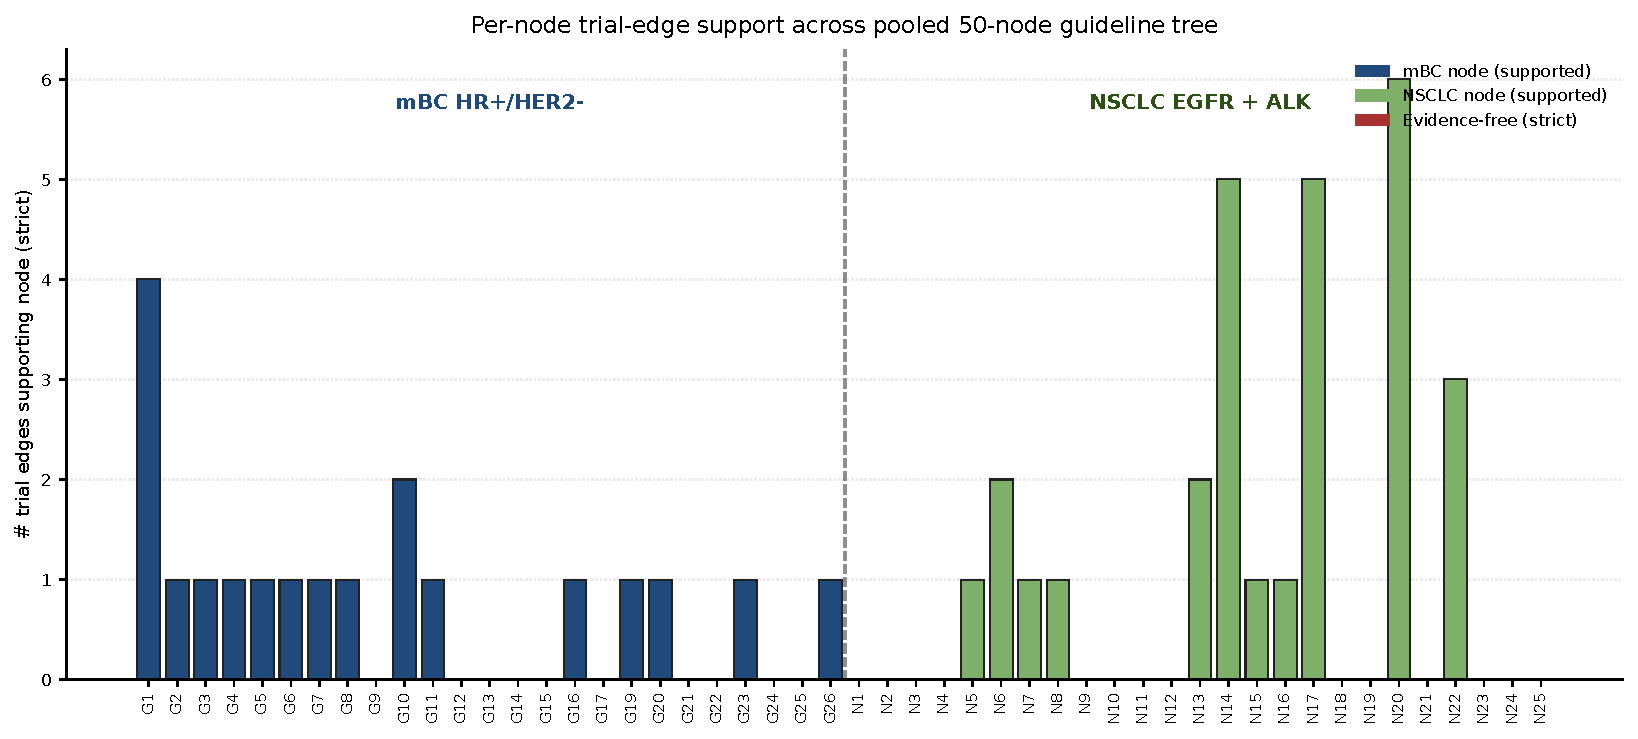
\includegraphics[width=0.95\linewidth]{../figures/v3_fig2_per_node.pdf}
\caption{Per-node trial-edge support across the NSCLC EGFR + ALK decision tree (24 nodes). Red bars: evidence-free under strict concordance. Compare clusters at post-osimertinib EGFR (5 of 7 evidence-free) versus first-line ALK (well-covered). The mBC nodes shown to the left of the divider are reproduced from the parallel multi-tumor pooled analysis for visual reference only and are not part of this NSCLC-only inference.}
\label{fig:per_node}
\end{figure}

\subsection{Operationalization discordance}
On the 178-trial NSCLC corpus, the prior-EGFR-TKI inclusion variable showed substantial cross-trial discordance (some trials require prior 1st/2nd-gen TKI progression, some require post-osimertinib, some permit either, some specify EGFR-resistance-window proxies). This operationalization heterogeneity is the structural reason the post-osimertinib decision nodes are difficult to support directly: subgroups derived from mixed-prior-TKI populations cannot be cleanly combined with subgroups from require-prior-osimertinib populations.

\section{Discussion}\label{sec:discussion}

\paragraph{Headline.}
On 24 unified ESMO+ASCO+NCCN NSCLC EGFR + ALK decision nodes against 147 in-scope trial edges, 9 (37.5\%) lacked any pivotal trial directly enrolling the (state, biomarker) population the guideline recommends. The post-osimertinib decision space is the most evidence-sparse single position in the modern guideline tree. The pre-registered exact-binomial test gave $P = 0.121$, one node below the critical value for rejection at $\alpha = 0.05$ — single-tumor scale ($n = 24$ nodes) is structurally under-powered for confirmatory binomial inference, and we present the findings as descriptive evidence plus framework demonstration rather than confirmatory rejection. A parallel multi-tumor pooled analysis (mBC + NSCLC) reported in a companion manuscript reaches confirmatory rejection at $P = 0.023$ at $n = 49$ pooled nodes.

\paragraph{What this means for clinicians and trial sponsors.}
The post-osimertinib decision space (where N7--N9, N21, N23 are evidence-free under strict concordance) is exactly where the next generation of pivotal trials should target enrichment populations: post-osimertinib pure cohorts, stratified by MET amplification and HER3 expression, with formal post-amivantamab arms. The MARIPOSA-2 / HERTHENA-Lung01 / TROPION-Lung01 / SAVANNAH evidence base is not absent --- it is just structured around mixed-prior-TKI populations and subgroup readouts that do not strictly match the guideline-encoded patient state.

\paragraph{Why ALK looks different.}
The ALK-rearranged decision tree was specifically built around line-of-therapy stratification (1L $\to$ 2nd-gen ALK TKI; post-1st-gen $\to$ 2nd-gen; post-2nd-gen $\to$ lorlatinib). ALEX, ALTA-1L, CROWN, and PROFILE 1014 enrolled clean first-line populations; post-progression trials use defined-stratum designs. EGFR-mutant trials, in contrast, have grown around osimertinib as the first-line standard but post-osimertinib trials have often used permissive eligibility (any prior EGFR TKI). The contrast between EGFR (fragmented) and ALK (consolidated) inside the same tumor type and the same framework is itself the strongest validation that the framework measures real structural differences in evidence landscapes.

\paragraph{Three caveats.}
First, $n = 24$ NSCLC nodes is under-powered for the binomial test; a single guideline-node flip moves $P$ from 0.121 to 0.049. The single-tumor descriptive framing is therefore the correct primary read. Second, the LLM-extraction pipeline failed the $\kappa \ge 0.70$ gate pre-adjudication on \texttt{post\_alk\_tki}, \texttt{egfr\_t790m}, and \texttt{drug\_class}; we disclose this honestly and a formal NSCLC adjudication pass is deferred. Third, the v3 corpus excludes HER2-mutated NSCLC, KRAS G12C, ROS1, RET, MET ex14, NTRK, and BRAF V600E by pre-specified scope; their inclusion would expand the decision tree by a further $\sim$10 nodes but is left to a future driver-broad extension.

\paragraph{Three positives.}
First, the framework is fully reproducible from the public ClinicalTrials.gov API; the 702-candidate $\to$ 178-trial filter pipeline, the 24-node decision-tree encoding, and the dual-annotator extraction outputs are released open-source. Second, the ALK falsifiability demonstration shows that the framework discriminates fragmented from consolidated evidence landscapes. Third, the post-osimertinib gap is concrete and immediately actionable: the trial agenda already underway (MARIPOSA-2, HERTHENA-Lung01, TROPION-Lung01, SAVANNAH next-generation studies) can be designed with the precise (state, biomarker) target populations our overlay identifies.

\paragraph{Limitations.}
Single-tumor scale limits binomial-test power. Hand-curated NSCLC guideline encoding by one author; a clinical second-annotator pass is deferred. Corpus snapshot at freeze 2026-05-16 excludes trials primarily completing after 2026. NCT-misidentification corrections were applied across two internal review rounds (four corrected, one dropped) and are documented in the supplement.

\paragraph{Outlook.}
The released framework supports continuous EFDPR auditing at each ESMO/ASCO/NCCN guideline update. A multi-tumor pooled extension (mBC + NSCLC) achieves confirmatory rejection ($P = 0.023$) and is reported separately; expansion to mCRC and other biomarker-driven solid tumors will further increase power. For NSCLC specifically, the priority is a clinical second-annotator pass on the 24-node tree, formal NSCLC adjudication rules, and integration of driver-broad subtypes (HER2-mut, KRAS G12C, ROS1, RET, MET ex14) into a v4 extension.

\subsection*{Data and code availability}
ClinicalTrials.gov queries reproduced in \texttt{analysis/v3\_01\_systematic\_search\_nsclc.py}; guideline decision-tree encoding, structured trial corpus, dual-annotator extractions, and adjudication-rule logs released under MIT licence at \url{https://github.com/htlin/mbc-evidence-dag-paper} at tag \texttt{v3.1.0}; Zenodo DOI minted at release.

\subsection*{Pre-registration}
\texttt{docs/prereg-v3.md} at commit \texttt{4b5bf1a}, committed before any NSCLC outcome-touching analysis. Companion methods preprint at medRxiv [DOI pending].

\subsection*{Author contributions (CRediT)}
\textbf{H.-T.\ Lin}: Conceptualization, Methodology, Software, Formal analysis, Investigation, Data curation, Validation, Visualization, Writing -- original draft, Writing -- review \& editing.

\subsection*{Conflicts of interest}
The author declares no competing financial or non-financial interests relevant to this work.

\subsection*{Funding}
No specific funding was received for this work.

\bibliographystyle{vancouver}
\bibliography{references}

\end{document}
